\section{Theorie}\label{sec:theorie}
Nachdem zunächst auf die verschiedenen Wechselwirkungen von elektromagnetischer Strahlung mit Materie eingegangen wird, folgt mit diesem Wissen eine Einführung in die Funktionsweise des verwendeten Germaniumdetektors.
\subsection{Wechselwirkungsprozesse von Photonen mit Materie}
Im Wesentlichen spielen drei Effekte eine wesentliche Rolle bei dem Einfall von im Versuch erzeugten Gammaquanten in Materie, wie in \autoref{fig:extinkt} dargestellt ist. Diese sind der Compton-Effekt, der Photoelektrische Effekt und die Paarerzeugung, wobei sich diese Effekte mit steigender Photonenenergie in ihrer Dominanz ablösen
Allgemein kann die Intensität $I$ von Strahlung innerhalb eines Materials abhängig von der Eindringtiefe $x$ mithilfe der Funktion
\begin{align}
  I(x) = I_0\cdot\exp{(-\mu x)}
\end{align}
modelliert werden, wobei $\mu$ Extinktionskoeffizient oder Absorptionskoeffizient genannt wird. Dieser von verschiedenen Materialeigenschaften sowie Strahlungsenergie abhängige Paramater beschreibt, wie stark ein Material die respektive Strahlung abschwächt.
Im Anschließenden wird der zustandekommende Graph erklärt.
\begin{figure}[H]
  \centering
  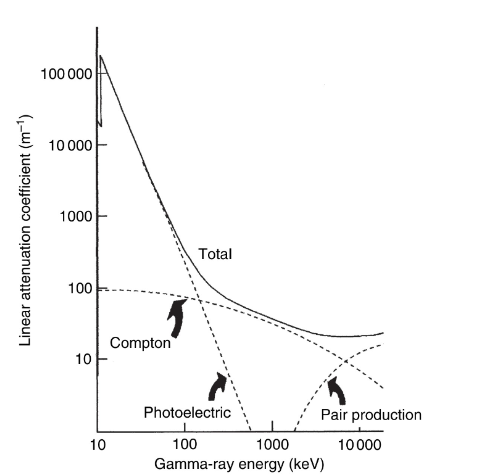
\includegraphics[scale=0.65]{Ressourcen/extinkt.png}
  \caption{Schematischer Verlauf des Extinktionskoeffizienten in Abhängigkeit der Photonenenergie\cite{gilmore}.}
  \label{fig:extinkt}
\end{figure}
\subsubsection{Photoelektrischer Effekt}
Der Photoeffekt beschreibt den Prozess, bei dem ein Gammaquant seine gesamte Energie an ein Hüllelektron eines Atoms abgibt, es herauslöst und das Atom somit ionisiert. Damit es zu diesem Verhalten kommen kann, müssen die Photonen bestimmte Energien, welche mit den Bindungsenergien der Elektronen im Atom übereinstimmen, besitzen.
Der Wirkungsquerschnitt $\sigma$, ein Maß für die Wahrscheinlichkeit eines Wechselwirkungsprozesses, sinkt für den Photoelektrischen Effekt mit steigender Energie, was sich in \autoref{fig:extinkt} in einer Abnahme des Extinktionskoeffizienten $\mu$ widerspiegelt.
Konkret ergibt sich als quantitative Abhängigkeit 
\begin{align}
  \sigma \sim Z^\alpha E^\delta\text{,}
\end{align}
wobei $Z$ die Kernladungszahl des Absorbers, $E$ die Strahlungsenergie und $\alpha \in(4,5)$ und $\delta = -3,5$ die Exponenten der Proportionalität beschreiben.
Ebenso ist ersichtlich, dass dieser Prozess für Photonenenergien bis zu $\SI{100}{\kilo\electronvolt}$ dominiert.

\subsubsection{Compton-Effekt}
Ebenso können Photonen an Hüllenelektronen im Korpuskelmodell des Lichts unelastisch gestreut werden und so ein Energieübertrag geleistet werden, wodurch sich die Wellenlänge des Photons verlängert. Im Gegensatz zum Photoeffekt wird bei diesem Prozess nur ein Teil der Energie übertragen und das Photon kann den Absorber wieder verlassen.
Als Abhängigkeit der Energie des gestreuten Photons $E_\gamma'$ von der Energie des einfallenden Photons $E_\gamma$ und dem Streuwinkel $\theta$, mit Annahme eines ruhenden Elektrons ergibt sich
\begin{align}
  E_\gamma' = \frac{E_\gamma}{1+\frac{E_\gamma}{m_0c^2}(1-\cos{\theta})}\text{,}\label{eqn:compton}
\end{align}
wobei $m_0$ die Ruhemasse des Elektrons und $c$ die Lichtgeschwindigkeit beschreibt.
Aus \autoref{eqn:compton} ist ersichtlich, dass der maximale Energieübertrag von Photon auf Elektron
\begin{align}
  E_{\text{max}} = E_\gamma\left(1-\frac{1}{1+\frac{2E_\gamma}{m_0c^2}}\right)\label{eqn:Comptonmax}
\end{align}
bei einem Streuwinkel von $\SI{180}{\degree}$ stattfindet.
Die quantitative Beschreibung der Winkelverteilung der gestreuten Photonen erfolgt durch die Klein-Nishina-Formel, welche den differentiellen Wirkungsquerschnitt nach dem Raumwinkel \(d\Omega\) angibt:
\begin{align}
  \frac{d\sigma}{d\Omega} = \frac{r_e^2}{2 [1 + \epsilon (1 - \cos \theta)]^2} \left( 1 + \cos^2 \theta + \frac{\epsilon^2 (1 - \cos \theta)^2}{1 + \epsilon (1 - \cos \theta)} \right) \label{eq:klein_nishina_dOmega}
\end{align}
Hierbei ist \(\theta\) der Streuwinkel des Photons, \(r_e = \frac{e_0}{4\pi\epsilon_0c^2m_0}\) der klassische Elektronenradius und \(\epsilon = E_\gamma / (m_e c^2)\) die auf die Elektronenruheenergie normierte Energie des einfallenden Photons \(E_\gamma\). Der totale Compton-Wirkungsquerschnitt ergibt sich durch Integration dieser Formel über den gesamten Raumwinkel.

Für die Analyse der Energieverteilung, insbesondere der an das Elektron übertragenen Energie \(E_e = E_\gamma - E\), ist der differentielle Wirkungsquerschnitt in Abhängigkeit der Energie \(E\) des gestreuten Photons relevant. Dieser ergibt sich zu:
\begin{align}
  \frac{d\sigma}{dE} = \frac{\pi r_e^2}{\epsilon E_\gamma} \left( 2 - \frac{2E}{\epsilon (E_\gamma - E)} + \frac{E^2}{\epsilon^2 (E_\gamma - E)^2} + \frac{E^2}{E_\gamma (E_\gamma - E)} \right) \label{eqn:Wirkungsquerschnitt}
\end{align}
Wird der Wirkungsquerschnitt pro Atom unter der Annahme von freien Elektronen betrachtet, gilt die Abhängigkeit
\begin{align}
  \sigma_\text{Compton}^\text{Atom}=Z\cdot \sigma_\text{Compton}\text{.}
\end{align}
\subsubsection{Paarerzeugung}
Die letzte hier erwähnte Wechselwirkung ist die Paarerzeugung, bei welcher ein Photon im Coulomb Feld des Atomkerns in ein Elektron-Positron Paar umgewandelt wird.
Somit muss, um Paarerzeugung zu ermöglichen, für die Energie des Photons
\begin{align}
  E_\gamma \approx 2m_ec^2
\end{align}
gelten. Gemäß \autoref{fig:extinkt} dominiert dieser Prozess für Gamma-Quant-Energien größer als $\SI{1.022}{\mega\eV}$.
\subsection{Funktionsweise des Germaniumdetektors}
Halbleiterdetektoren, wie der im Versuch verwendete Germanium-Detektor, sind wichtige Instrumente zur Detektion und Analyse von Gammastrahlung. Ihre Funktion basiert auf den physikalischen Eigenschaften von Halbleitermaterialien und der oben beschriebenen Wechselwirkung der Gammastrahlung mit Materie. Im Folgenden wird die Funktionsweise eines Halbleiterdetektors beschrieben.

\subsubsection{Grundlagen}
Ein Halbleiterdetektor besteht im wesentlichen aus einer Halbleiterdiode, die aus zwei benachbarten Zonen besteht: einer \textit{n-dotierten} und einer \textit{p-dotierten} Zone, in welcher Atome mit relativ höherer oder niedrigerer Elektronenzahl ins Material eingebracht sind. 
An der Grenzfläche zwischen diesen beiden Zonen bildet sich durch Diffusion von Ladungsträgern eine sogenannte Verarmungszone, in der fast keine freien Ladungsträger vorhanden sind, wie in \autoref{fig:halb} links zu sehen ist. Um den Detektor betriebsbereit zu machen, wird eine äußere Spannung UU in Sperrrichtung angelegt. Diese Spannung erweitert die Verarmungszone, wie in \autoref{fig:halb} rechts dargestellt. Die \textit{Depletionsspannung} ist die spezifische Sperrspannung, die erforderlich ist, um die Verarmungszone über das gesamte aktive Volumen des Detektors auszudehnen, sodass einfallende Strahlung effizient Elektron-Loch-Paare in diesem ladungsfreien Bereich erzeugen kann.
\begin{figure}[H]
  \centering
  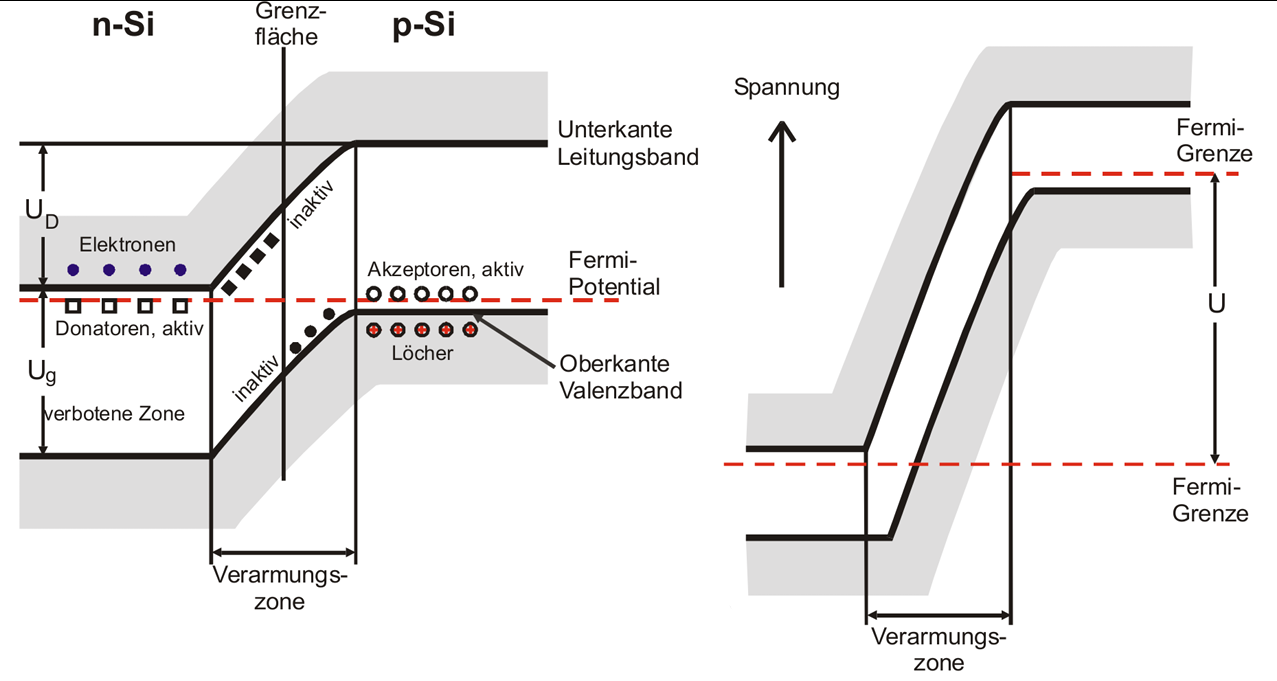
\includegraphics[scale=0.3]{Ressourcen/halbleiter.png}
  \caption{Prinzip des p-n-Übergangs als Detektor: Energiebänder ohne äußere Spannung (links) und mit angelegter Sperrspannung \(U\) (rechts), welche die für die Detektion notwendige Verarmungszone verbreitert. Bildquelle: \cite{anleitung}.}
  \label{fig:halb}
\end{figure}

\subsubsection{Wechselwirkung von Strahlung mit dem Detektor}
Trifft Gammastrahlung auf die Verarmungszone des Halbleiters und hat die Energie der Strahlung einen Wert oberhalb der Bandlücke des Materials, so können die Photonen Elektronen aus dem Valenzband in das Leitungsband anregen. Dies führt zur Bildung von Elektron-Loch-Paaren im Detektor. Die Anzahl dieser Paare ist proportional zur absorbierten Energie der Gammastrahlung:
\begin{align}
  n = \frac{E_{\text{abs}}}{\epsilon_\text{Paar}},
\end{align}
wobei $E_{\text{abs}}$ die Energie der absorbierten Strahlung und $\epsilon_\text{Paar}$ die Energie ist, die benötigt wird, um ein Elektron-Loch-Paar zu erzeugen.
Im Experiment wird der Germaniumdetektor mittels Helium auf etwa $\SI{80}{\kelvin}$ gekühlt, um das Auftreten von ungewollten thermisch angeregte Ladungsträger zu minimieren. Bei dieser Temperatur ergibt sich für Germanium eine Bandlücke von $\SI{0.73}{\eV}$\cite{Sze2007}.
\\Germanium ist ein \textit{indirekter Halbleiter}, was bedeutet, dass das Minimum des Leitungsbandes und das Maximum des Valenzbandes im Energie-Impuls-Diagramm bei unterschiedlichen \(k\)-Vektoren liegen, wie in \autoref{fig:indirekt} dargestellt. 
Für die Anregung eines Elektrons vom Valenz- ins Leitungsband durch ein Photon muss neben der Energie auch der Impuls erhalten bleiben. Da Photonen im Vergleich zu Elektronen im Kristallgitter nur einen sehr geringen Impuls tragen, kann die für den Übergang nötige Impulsänderung bei einem indirekten Halbleiter nicht allein durch das Photon erfolgen. 
Stattdessen ist die Wechselwirkung mit einer Gitterschwingung, einem Phonon, erforderlich, welches den fehlenden Impuls aufnimmt oder bereitstellt. Dieser Prozess (Photon + Elektron + Phonon) führt dazu, dass die minimale Energie zur Erzeugung eines Elektron-Loch-Paares zwar durch die Bandlücke gegeben ist, die durchschnittlich benötigte Energie jedoch höher liegt. Ein signifikanter Teil der Energie des einfallenden Teilchens geht in die Anregung von Gitterschwingungen verloren.
\begin{figure}[H]
  \centering
  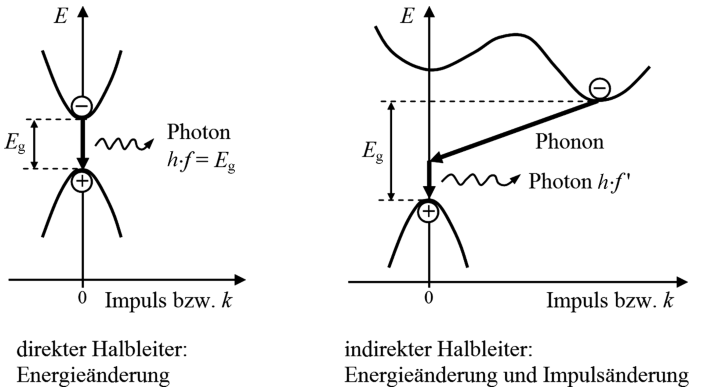
\includegraphics[scale=0.7]{Ressourcen/indirekt.png}
  \caption{Vergleich von Bandübergängen bei Halbleitern und indirekten Halbleitern.}
  \label{fig:indirekt}
\end{figure}
\subsection{Vollenergienachweiswahrscheinlichkeit}
Ein wichtiger Parameter zur Charakterisierung eines Germaniumdetektors ist die Vollenergienachweiswahrscheinlichkeit $Q$. Sie beschreibt die Wahrscheinlichkeit, dass ein von der Quelle emittiertes Gammaquant seine gesamte Energie im Detektor deponiert und somit zum Photopeak beiträgt. Diese Größe ist entscheidend für die quantitative Analyse von Gammaspektren und hängt von der Energie der Strahlung, der Detektorgeometrie und dem Detektormaterial ab.
Die Vollenergienachweiswahrscheinlichkeit kann durch folgende Formel ausgedrückt werden:
\begin{align}
  Q = \frac{N}{AW t} \cdot \frac{4\pi}{\Omega}\text{,}
\end{align}
wobei $N$ die Anzahl der im Photopeak registrierten Ereignisse, $A$ die Aktivität der Quelle, $W$ die Emissionswahrscheinlichkeit der betrachteten Gammalinie, $t$ die Messzeit und $\Omega$ der vom Detektor abgedeckte Raumwinkel ist.
Die Vollenergienachweiswahrscheinlichkeit nimmt typischerweise mit steigender Gammaenergie ab, da höherenergetische Photonen mit einer geringereen Wahrscheinlichkeit im Detektormaterial wechselwirken und häufiger den Detektor ohne vollständige Energiedeposition verlassen.
\subsubsection{Signalverarbeitung}
Die Elektronen bewegen sich aufgrund ihrer negativen Ladung und dem durch die angelegte Depletionsspannung erzeugten Elektrischen Feld zur $n$-Schicht, während die Löcher in Richtung der $p$-Schicht wandern. Auf dem Weg wechselwirken die Elektronen aufgrund ihrer hohen Energie weiter mit dem Detektor und erzeugen Sekundäre Elektron-Loch Paare. Dieser Ladungstransport erzeugt einen Strompuls, der durch eine komplexe elektronische Auslesekette verarbeitet wird, welche in \autoref{fig:schaltung} dargestellt ist.  Um thermische Anregung von Elektronen (Rauschen) zu minimieren, wird der Germaniumdetektor wie oben erwähnt mittels siedendem Helium gekühlt.
\begin{figure}[H]
  \centering
  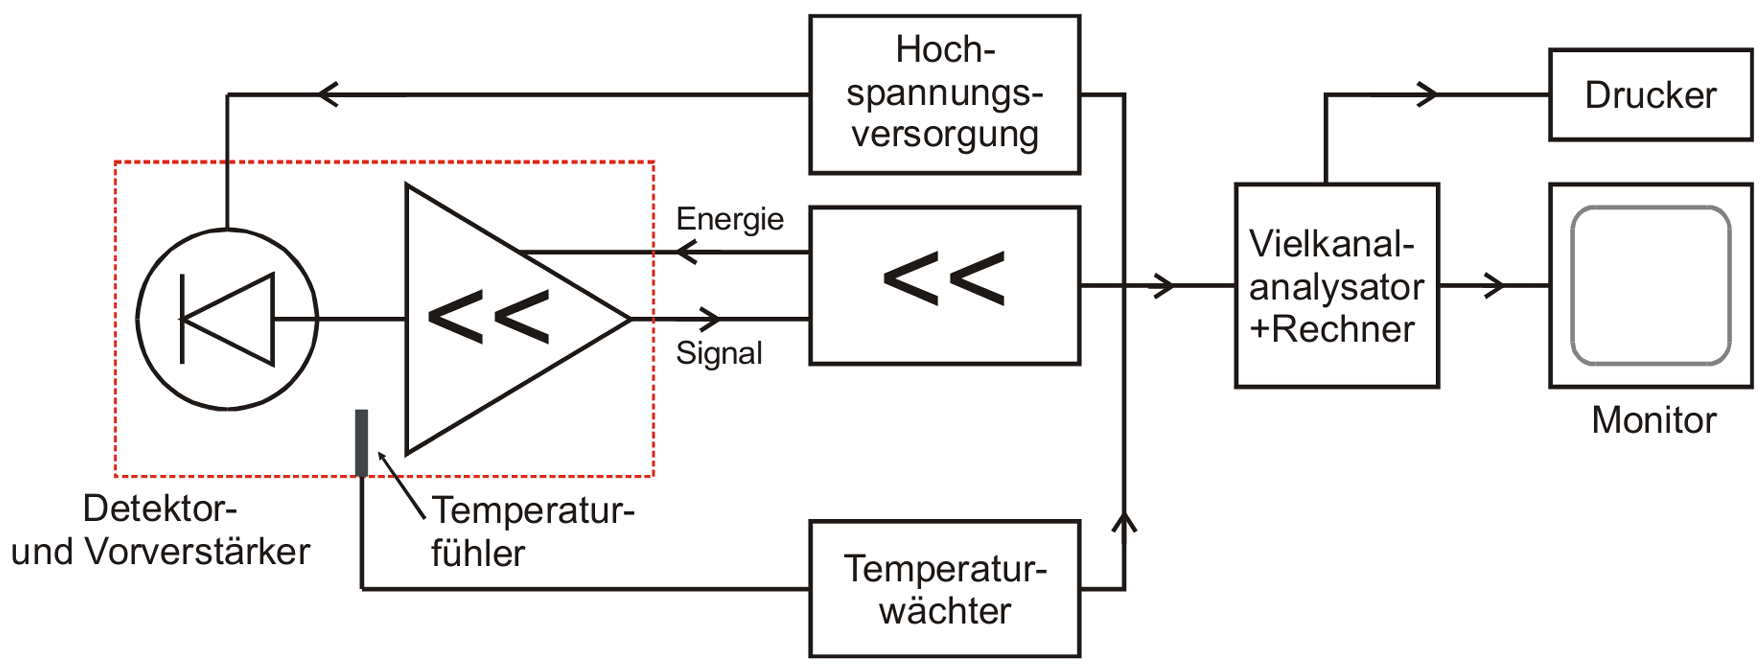
\includegraphics[scale=0.3]{Ressourcen/schaltung.png}
  \caption{Skizze der verwendeten Auslese-Schaltung.\cite{anleitung}}
  \label{fig:schaltung}
\end{figure}
Der Vorverstärker befindet sich in unmittelbarer Nähe zum Detektorkristall und wird mit diesem zusammen gekühlt, um Rauschspannungen zu minimieren. Er besteht wie in \autoref{fig:vorverstärker} visualisiert aus einem kapazitiv rückgekoppelten Operationsverstärker, dessen Ausgangspotential proportional zum integrierten Eingangsstrom ist. Bei Einfall mehrerer $\gamma$-Quanten führt dies zu einem stufenförmigen Anstieg der Ausgangsspannung. Um eine Analyse der einzelnen Pulshöhen zu ermöglichen, wird der Integrationskondensator durch eine optoelektronische Rückkopplung entladen.
\begin{figure}[H]
  \centering
  \includegraphics[scale=0.3]{Ressourcen/vorverstärker.png}
  \caption{Skizze des Vorverstärkers mit optoelektronischer Rückkopplung.\cite{anleitung}}
  \label{fig:vorverstärker}
\end{figure}
Der Vorverstärker ist über einen Hochpass an den Hauptverstärker gekoppelt, wobei eine sogenannte Pole-Zero-Kompensation Unterschwinger im Signal verhindert. Im Hauptverstärker wird das Signal integriert und differenziert, um eine optimale Bandbreite zu gewährleisten. Nach der Verstärkung wird die Pulshöhe mit einem Analog-Digital-Wandler, welcher in \autoref{fig:analogkette} gemessen und die Daten an einen Vielkanal-Analysator weitergegeben, der die Anzahl der Pulse in Abhängigkeit von ihrer Höhe speichert.
\begin{figure}[H]
  \centering
  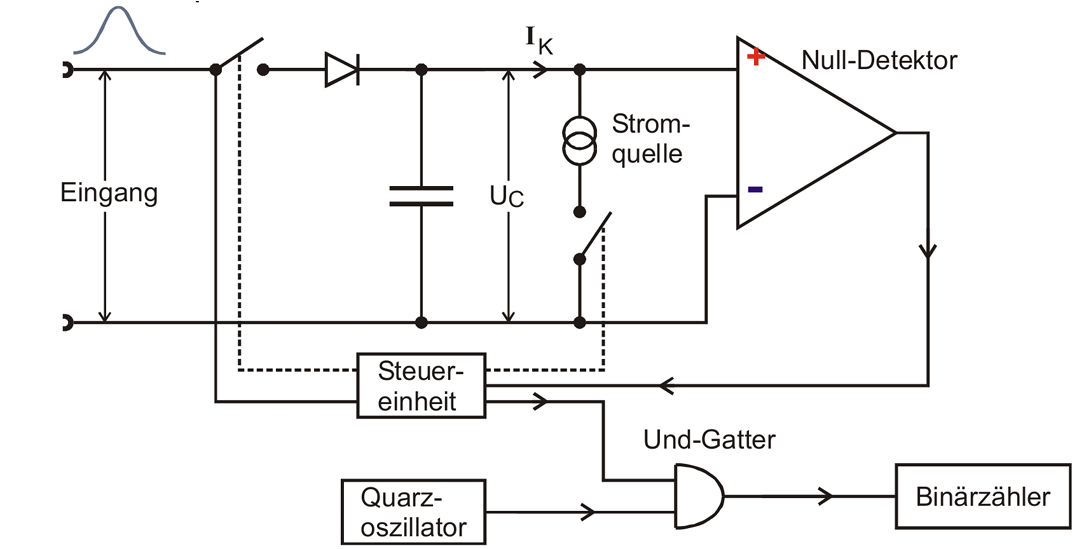
\includegraphics[scale=0.3]{Ressourcen/analogkette.png}
  \caption{Schaltbild des verwendeten Analog-Digital-Konverters.\cite{anleitung}}
  \label{fig:analogkette}
\end{figure}
Ein kritisches Problem bei der Signalverarbeitung ist das sogenannte Pile-up, welches auftritt, wenn mehrere Gammaquanten so kurz nacheinander im Detektor einfallen, dass ihre Signale zeitlich überlappen. Dies führt zu verfälschten Energiemessungen und einer Verschlechterung der Energieauflösung. Um dies zu vermeiden, wird die oben erwähnte optoelektronische Rückkopplung verwendet. Nach einem Impuls leuchtet eine LED auf den Eingangs-Feldeffekttransistor, wodurch dieser kurzzeitig leitend wird und eine schnelle Entladung des Integrationskondensators ermöglicht. Dadurch wird das System rasch für das nächste Ereignis vorbereitet. Zusätzlich wird nach der Verstärkung des Signals eine Totzeit eingehalten, während der keine weiteren Ereignisse verarbeitet werden. Der verwendete Wilkinson-Analog-Digital-Konverter hat eine typische Totzeit von etwa 40 µs, die sich aus einer konstanten Grundzeit und einer variablen Zeit proportional zur Pulshöhe zusammensetzt. Diese Maßnahmen zusammen ermöglichen eine präzise Energiemessung auch bei höheren Zählraten, indem sie sicherstellen, dass nahezu jedes Gammaquant individuell und korrekt verarbeitet wird.
\subsection{Spektrum eines monochromatischen Gamma-Strahlers}
Wie in \autoref{fig:cs137} beispielhaft für Cs-137 zu sehen, weist das Spektrum einer Gammaquelle mehrere charakteristische Stellen auf.
\begin{figure}[H]
  \centering
  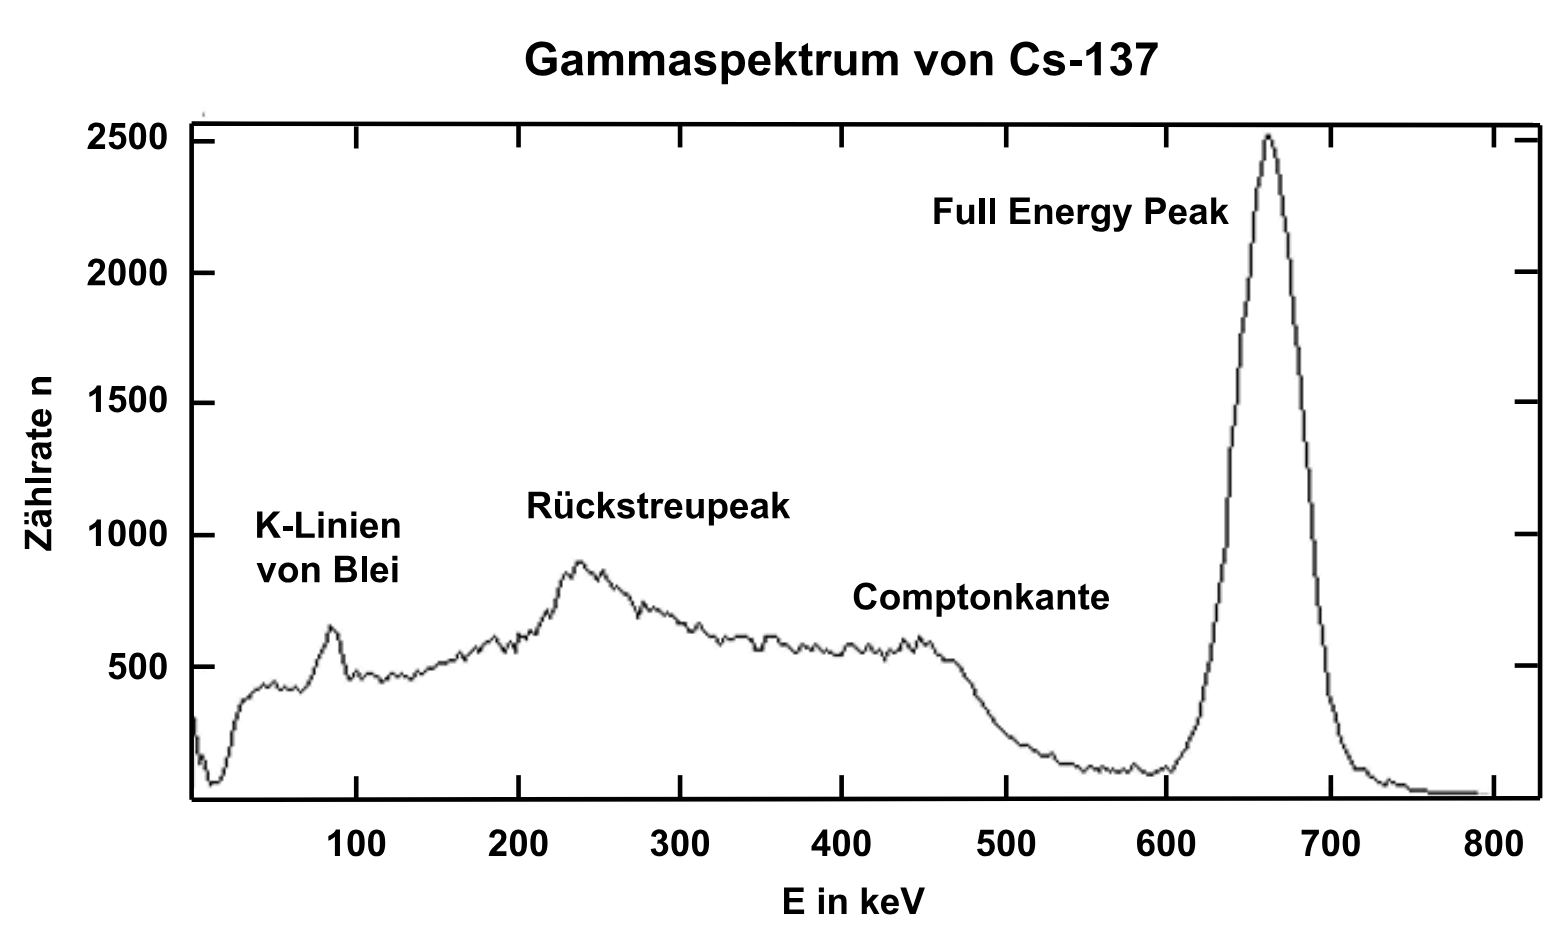
\includegraphics[scale=0.3]{Ressourcen/cs137.png}
  \caption{Spektrum einer Caesium-137 Quelle.\cite{leifics137}.}
  \label{fig:cs137}
\end{figure}
Wie oben erwähnt ist die Energiedeposition durch Compton-Streuung nicht diskret, wodurch das im Spektrum sichbare Compton-Kontinuum entsteht. Dieses Erstreckt sich von $E_\text{min}$, festgelegt durch das verwendete Material des Halbleiterdetektors und die Qualität des Detektors bezüglisch Rauschen und Energieauflösung selbst, bis zur Compton-Kante
\begin{align} 
  E_\text{max}=\frac{E_\gamma\cdot2\epsilon}{1+2\epsilon}\text{,}\label{eqn:Emax}
\end{align}
wie aus \autoref{eqn:Comptonmax} hervorgeht. Im Versuchsfall liegt liegt $E_\text{min}$ bei etwa $\SI{40}{\kilo\eV}$.
Des weiteren ist der Rückstreupeak ein charakteristischer Bereich im Gammaspektrum, der durch Photonen entsteht, die außerhalb des Detektors durch den Compton-Effekt gestreut wurden und anschließend mit reduzierter Energie in den Detektor zurückkehren. Die Energie dieser Photonen kann durch die Formel
\begin{align} 
E_{\text{Rück}} = \frac{E_\gamma}{1 + \frac{2E_\gamma}{m_e c^2}}\label{eqn:Eback}
\end{align}
berechnet werden. Der Rückstreupeak erscheint im Spektrum unterhalb der Compton-Kante.
Der in \autoref{fig:cs137} prominenteste Full Energy Peak/ Photopeak steht für den Fall der restlosen Energiedeposition des Gammaquants durch den Photoeffekt, optional nach vorheriger Compton-Streuung. Der Peak repräsentiert somit direkt die Energie der einfallenden Gammaquanten. 